\documentclass[11pt,a4paper,oneside]{report}

% thanks to http://tex.stackexchange.com/a/47579/71109
\usepackage{pdfpages}
\usepackage{ifxetex}
\usepackage{ifluatex}
\newif\ifxetexorluatex % a new conditional starts as false
\ifnum 0\ifxetex 1\fi\ifluatex 1\fi>0
   \xetexorluatextrue
\fi

\ifxetexorluatex
  \usepackage{fontspec}
\else
  \usepackage[T1]{fontenc}
  \usepackage[utf8]{inputenc}
  \usepackage[lighttt]{lmodern}
  \ttfamily\DeclareFontShape{T1}{lmtt}{m}{it}{<->sub*lmtt/m/sl}{}
\fi

\usepackage[english,magyar]{babel} % Alapértelmezés szerint utoljára definiált nyelv lesz aktív, de később külön beállítjuk az aktív nyelvet.

\usepackage{emptypage} % omit page number on empty pages

%\usepackage{cmap}
\usepackage{amsfonts,amsmath,amssymb} % Mathematical symbols.
%\usepackage[ruled,boxed,resetcount,linesnumbered]{algorithm2e} % For pseudocodes. % beware: this is not compatible with LuaLaTeX, see http://tex.stackexchange.com/questions/34814/lualatex-and-algorithm2e
\usepackage{booktabs} % For publication quality tables for LaTeX
\usepackage{graphicx}

%\usepackage{fancyhdr}
%\usepackage{lastpage}

\usepackage{anysize}
%\usepackage{sectsty}
\usepackage{setspace} % For setting line spacing

\usepackage[unicode]{hyperref} % For hyperlinks in the generated document.
\usepackage{xcolor}
\usepackage{listings} % For source code snippets.

\usepackage[amsmath,thmmarks]{ntheorem} % Theorem-like environments.

\usepackage[hang]{caption}

\singlespacing

\newcommand{\selecthungarian}{
	\selectlanguage{magyar}
	\setlength{\parindent}{2em}
	\setlength{\parskip}{0.5em}
	\frenchspacing
}

\newcommand{\selectenglish}{
	\selectlanguage{english}
	\setlength{\parindent}{0em}
	\setlength{\parskip}{0.5em}
	\nonfrenchspacing
	\renewcommand{\figureautorefname}{Figure}
	\renewcommand{\tableautorefname}{Table}
	\renewcommand{\partautorefname}{Part}
	\renewcommand{\chapterautorefname}{Chapter}
	\renewcommand{\sectionautorefname}{Section}
	\renewcommand{\subsectionautorefname}{Section}
	\renewcommand{\subsubsectionautorefname}{Section}
}

\usepackage[numbers]{natbib}
\usepackage{xspace}


\newcommand{\vikszerzoVezeteknev}{Fintha}
\newcommand{\vikszerzoKeresztnev}{Dénes Flórián}

\newcommand{\vikkonzulensAMegszolitas}{Dr.~}
\newcommand{\vikkonzulensAVezeteknev}{Bergmann}
\newcommand{\vikkonzulensAKeresztnev}{Gábor}

\newcommand{\vikkonzulensBMegszolitas}{}
\newcommand{\vikkonzulensBVezeteknev}{}
\newcommand{\vikkonzulensBKeresztnev}{}

\newcommand{\vikkonzulensCMegszolitas}{}
\newcommand{\vikkonzulensCVezeteknev}{}
\newcommand{\vikkonzulensCKeresztnev}{}

\newcommand{\vikcim}{Performance analysis of a language tooling}
\newcommand{\viktanszek}{\bmemit}
\newcommand{\vikdoktipus}{\bsc}
\newcommand{\vikmunkatipusat}{szakdolgozatot}

\newcommand{\szerzoMeta}{\vikszerzoVezeteknev{} \vikszerzoKeresztnev}
\input{include/thesis-en}
%--------------------------------------------------------------------------------------
% Page layout setup
%--------------------------------------------------------------------------------------
% we need to redefine the pagestyle plain
% another possibility is to use the body of this command without \fancypagestyle
% and use \pagestyle{fancy} but in that case the special pages
% (like the ToC, the References, and the Chapter pages)remain in plane style

\pagestyle{plain}
\marginsize{35mm}{25mm}{15mm}{15mm}

\setcounter{tocdepth}{3}
%\sectionfont{\large\upshape\bfseries}
\setcounter{secnumdepth}{3}

\sloppy % Margón túllógó sorok tiltása.
\widowpenalty=10000 \clubpenalty=10000 %A fattyú- és árvasorok elkerülése
\def\hyph{-\penalty0\hskip0pt\relax} % Kötőjeles szavak elválasztásának engedélyezése


%--------------------------------------------------------------------------------------
% Setup hyperref package
%--------------------------------------------------------------------------------------
\hypersetup{
    % bookmarks=true,            % show bookmarks bar?
    unicode=true,              % non-Latin characters in Acrobat's bookmarks
    pdftitle={\vikcim},        % title
    pdfauthor={\szerzoMeta},    % author
    pdfsubject={\vikdoktipus}, % subject of the document
    pdfcreator={\szerzoMeta},   % creator of the document
    pdfproducer={},    % producer of the document
    pdfkeywords={},    % list of keywords (separate then by comma)
    pdfnewwindow=true,         % links in new window
    colorlinks=true,           % false: boxed links; true: colored links
    linkcolor=black,           % color of internal links
    citecolor=black,           % color of links to bibliography
    filecolor=black,           % color of file links
    urlcolor=black             % color of external links
}


%--------------------------------------------------------------------------------------
% Set up listings
%--------------------------------------------------------------------------------------
\definecolor{lightgray}{rgb}{0.95,0.95,0.95}
\lstset{
	basicstyle=\scriptsize\ttfamily, % print whole listing small
	keywordstyle=\color{black}\bfseries, % bold black keywords
	identifierstyle=, % nothing happens
	% default behavior: comments in italic, to change use
	% commentstyle=\color{green}, % for e.g. green comments
	stringstyle=\scriptsize,
	showstringspaces=false, % no special string spaces
	aboveskip=0.5em,
	belowskip=0.5em,
	backgroundcolor=\color{lightgray},
	columns=flexible,
	keepspaces=true,
	escapeinside={(*@}{@*)},
	captionpos=b,
	breaklines=true,
	frame=single,
	float=!ht,
	tabsize=2,
	literate=*
		{á}{{\'a}}1	{é}{{\'e}}1	{í}{{\'i}}1	{ó}{{\'o}}1	{ö}{{\"o}}1	{ő}{{\H{o}}}1	{ú}{{\'u}}1	{ü}{{\"u}}1	{ű}{{\H{u}}}1
		{Á}{{\'A}}1	{É}{{\'E}}1	{Í}{{\'I}}1	{Ó}{{\'O}}1	{Ö}{{\"O}}1	{Ő}{{\H{O}}}1	{Ú}{{\'U}}1	{Ü}{{\"U}}1	{Ű}{{\H{U}}}1
}


%--------------------------------------------------------------------------------------
% Set up theorem-like environments
%--------------------------------------------------------------------------------------
% Using ntheorem package -- see http://www.math.washington.edu/tex-archive/macros/latex/contrib/ntheorem/ntheorem.pdf

\theoremstyle{plain}
\theoremseparator{.}
\newtheorem{example}{\pelda}

\theoremseparator{.}
%\theoremprework{\bigskip\hrule\medskip}
%\theorempostwork{\hrule\bigskip}
\theorembodyfont{\upshape}
\theoremsymbol{{\large \ensuremath{\centerdot}}}
\newtheorem{definition}{\definicio}

\theoremseparator{.}
%\theoremprework{\bigskip\hrule\medskip}
%\theorempostwork{\hrule\bigskip}
\newtheorem{theorem}{\tetel}


%--------------------------------------------------------------------------------------
% Some new commands and declarations
%--------------------------------------------------------------------------------------
\newcommand{\code}[1]{{\upshape\ttfamily\scriptsize\indent #1}}
\newcommand{\doi}[1]{DOI: \href{http://dx.doi.org/\detokenize{#1}}{\raggedright{\texttt{\detokenize{#1}}}}} % A hivatkozások közt így könnyebb DOI-t megadni.

\DeclareMathOperator*{\argmax}{arg\,max}
%\DeclareMathOperator*[1]{\floor}{arg\,max}
\DeclareMathOperator{\sign}{sgn}
\DeclareMathOperator{\rot}{rot}


%--------------------------------------------------------------------------------------
% Setup captions
%--------------------------------------------------------------------------------------
\captionsetup[figure]{aboveskip=10pt}

\renewcommand{\captionlabelfont}{\bf}
%\renewcommand{\captionfont}{\footnotesize\it}

%--------------------------------------------------------------------------------------
% Hyphenation exceptions
%--------------------------------------------------------------------------------------
\hyphenation{Shakes-peare Mar-seilles ár-víz-tű-rő tü-kör-fú-ró-gép}


\author{\vikszerzo}
\title{\viktitle}


\begin{document}


\includepdf[pages=-]{include/feladatkiiras.pdf}
\clearpage

\pagenumbering{gobble}
\selectthesislanguage
\hypersetup{pageanchor=false}
%--------------------------------------------------------------------------------------
%	The title page
%--------------------------------------------------------------------------------------
\begin{titlepage}
\begin{center}
\includegraphics[width=60mm,keepaspectratio]{figures/bme_logo.pdf}\\
\vspace{0.3cm}
\textbf{\bme}\\
\textmd{\vik}\\
\textmd{\viktanszek}\\[5cm]

\vspace{0.4cm}
{\huge \bfseries \vikcim}\\[0.8cm]
\vspace{0.5cm}
\textsc{\Large \vikdoktipus}\\[4cm]

{
	\renewcommand{\arraystretch}{0.85}
	\begin{tabular}{cc}
	 \makebox[7cm]{\emph{\keszitette}} & \makebox[7cm]{\emph{\konzulens}} \\ \noalign{\smallskip}
	 \makebox[7cm]{\szerzo} & \makebox[7cm]{\vikkonzulensA} \\
	  & \makebox[7cm]{\vikkonzulensB} \\
	  & \makebox[7cm]{\vikkonzulensC} \\
	\end{tabular}
}

\vfill
{\large December 10, 2020}
\end{center}
\end{titlepage}
\hypersetup{pageanchor=false}


\tableofcontents\cleardoublepage
\include{include/declaration}

% --- ABSTRACT --------------------------------------------------------------- %

\pagenumbering{roman}
\setcounter{page}{1}

\selecthungarian
\chapter*{Kivonat}\addcontentsline{toc}{chapter}{Kivonat}
A szakdolgozat egy modellek validációjával foglalkozó eszköz teljesítményével
kapcsolatos problémáinak nyomozásáról és orvoslásáról szól.

A vizsgált eszköz a VIATRA Query, melyben mintákat definiálhatunk, és
illeszthetünk modellekre az esetleges hibák felderítésére, egy kifejezetten erre
szolgáló nyelv segítségével (VIATRA Query Language, VQL). A közelmúltban több
felhasználónak is feltűnt, hogy a VQL szerkesztő indokolatlanul lassan reagál
a lekérdezések szerkesztésére, mely megakadályozza a gördülékeny munkamenetet.

A dolgozatban nagy vonalakban ismertetem a VIATRA Query-t, mint szoftvert,
valamint mutatok néhány egyszerű példát a használatára minták írásán keresztül.

A szoftver bemutatása után egy ismerten lassú példafájl használatával bemutatom
a probléma forrásának felderítését egy profilozó szoftver segítségével. Emellett
részletekbe menően ismertetem a releváns részek működését, valamint kidolgozok
egy potenciális javítást is.

Végül miután elkészült a javítás, utolsó lépésként bemutatom, hogyan lehet a
változtatásokat elküldeni a VIATRA fejlesztőinek, hogy a szoftver következő
kiadása már tartalmazhassa őket.
\vfill

\selectenglish
\chapter*{Abstract}\addcontentsline{toc}{chapter}{Abstract}
This thesis is about investigating and solving the performance issues of a tool,
which validates models.

The tool we inspect is VIATRA Query, in which we can define patterns, and match
them on models to check them for potential errors. This is done in a
domain-specific language (VIATRA Query Language, VQL). In the past, multiple
users have noticed, that the VQL editor reacts in an unreasonably slow manner to
changes in the VQL editor, which obstructs a smooth workflow.

In the thesis, I'll broadly show the VIATRA Query software, and show the
basic usage of it through some simple patterns.

After showing the tool itself, I'll present the investigation of the problem by
using a file, that is known to cause slowdowns, and a profiler software. Along
with this, I'll show the details about how that part of the software works, and
work out a potential fix for it, too.

Finally, after the my fix is in a working state, I'll show how to send changes
to the developers of VIATRA, so my fix could be included in its next release.
\vfill

% ---------------------------------------------------------------------------- %

\cleardoublepage
\selectthesislanguage
\newcounter{romanPage}
\setcounter{romanPage}{\value{page}}
\stepcounter{romanPage}
\pagenumbering{arabic}

% --- CONTENT ---------------------------------------------------------------- %

\chapter{Introduction}

\section{The VIATRA framework}
VIATRA (VIsual Automated model TRAnsformations) is an open-source project backed
by the Eclipse Foundation, which integrates into the Eclipse development
environment, providing functionalities like obfuscation, transformation, and
query of models.

In my thesis, I worked with the VIATRA Query component, which is a tool for
writing and executing queries on models in the context of the discipline of
model-based engineering.

\begin{figure}[ht]
\centering
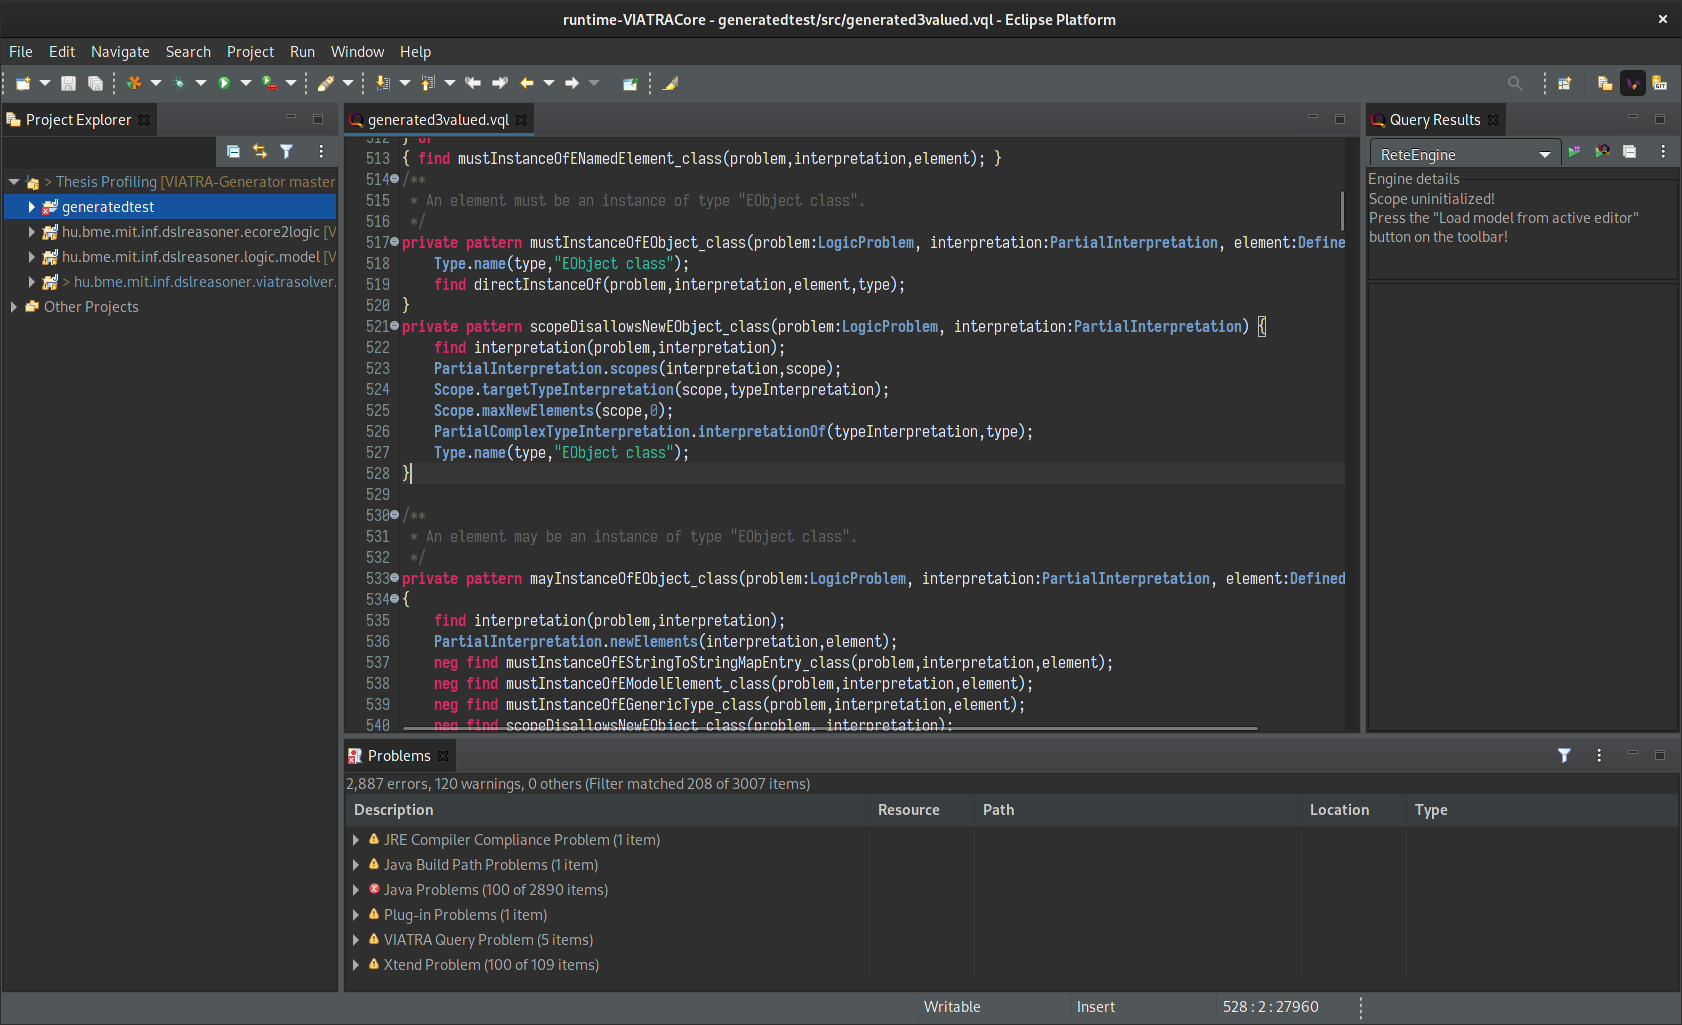
\includegraphics[width=150mm, keepaspectratio]{figures/eclipse-viatra.png}
\caption{The VIATRA Transformation Development perspective in Eclipse}
\label{fig:eclipse-viatra}
\end{figure}

\section{VIATRA Query Language (VQL)}
An effective way of validating models is declaring patterns indicating incorrect
models. For example, if our model represents a family tree, we may look for
cycles.

In VIATRA Query, we can write such patterns that are matched on a loaded model.
Defining patterns is done via a powerful domain-specific language (DSL) called
the VIATRA Query Language (VQL). The VIATRA Query Eclipse plugins provide an
editor with proper syntax highlighting and code completion to make writing
patterns easier.

\section{VQL editor slowdowns}
Users have noticed, that the VQL editor is, in some cases inexplicably slow.
As such, for this issue, a bugzilla ticket was already opened by the
community\cite{bugzilla-ticket}.

During my manual tests, editing some queries frequently caused 5 to 10 second
hangups. This notably happens during a process called ``Xtext validation''.

\chapter{Background}

\section{Domain-specific modeling and metamodels}
Domain-specific modeling is a methodology, which uses models to represent
systems, mostly by using domain-specific languages (DSL). Often these models
are then subject to code generation, translating the model of a system to a
program representing that system.

The entities and relations of these models are described by their
\textbf{metamodels}, which preactically act as schemas for them, defininf the
entities and relations in the model. For example, if our model represents a
family tree, we may have \texttt{Person} entities, and \texttt{mother} and
\texttt{father} relations between them.

\section{Eclipse plug-in development}
Eclipse is an integrated development environment (IDE), which can be customized
with plug-ins. These plug-ins extend the functionality of Eclipse, and can have
various roles, such as providing support for development in a programming
language, or integrating the use of an external tool to our workflow.

During plug-in development, the \textbf{target platform} is the Eclipse
environment we build our plug-in to work with. These plug-ins may contain
the metamodel(s) for the models managed by them, such as the metamodel for a
system or even a domain-specific language.

In my case, VIATRA itself is a bundle of Eclipse plug-ins, providing a query
development environment with an editor and a code generator for model
queries, which includes the metamodel for VQL\cite{viatra}.

Integration of the YourKit Java Profiler is also done through a plug-in, which
lets me run the software in profiling mode, and configure the profiler itself
in Eclipse.

\section{The Xtext language framework}
VQL was implemented using the Xtext framework. This framework is an effective
tool for developing programming and domain-based languages.

For the languages implemented using it, the Xtext framework provides the
following services\cite{xtext}.

\begin{itemize}
    \item{language parser}
    \item{linker}
    \item{editing support in editors supporting the Language Server Protocol}
    \item{
        customizable language services, which one can build their concrete
        implementation on
        \begin{itemize}
            \item{scoping}
            \item{validation}
            \item{code generation}
            \item{outline support}
        \end{itemize}
    }
    \item{the Xbase expression language library}
\end{itemize}

It should also be noted, that some internal parts of VQL infrastructure were
implemented using the Xtend language, which is also part of the Xtext project,
implemented in Xtext itself. Xtend is a Java dialect, with some modern language
elements, such as macros, lambdas, and operator overloading\cite{xtend}.

\section{Query language syntax}
VQL is a datalog dialect, which means that instead of writing functions, we
write statements, which are solved on our model. The engine will try to match
the pattern on the model, and show each match in it.

\subsection{Writing patterns}
Patterns begin with the \texttt{pattern} keyword, followed by the name of our
pattern, and its parameter list. The body of a pattern contains statements,
which can use existing parameters, and introduce new ones.

This simple pattern will match each grandparent-grandchild relation in a model,
which contains \texttt{Node}s, with one parent each.

\begin{lstlisting}[caption={Grandparent-grandchild relation for \texttt{Node}s}, frame=single]
pattern grandparentOf(grandchild : Node, grandparent : Node) {
    Node.parent(grandchild, parent);
    Node.parent(parent, grandparent);
}
\end{lstlisting}

We have two \texttt{Node} entities, \texttt{grandchild} and
\texttt{grandparent}. These come from the parameters of the pattern.

\begin{figure}[!htbp]
\centering
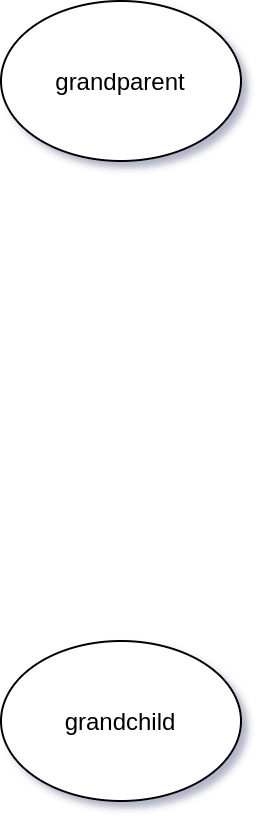
\includegraphics[height=50mm, keepaspectratio]{figures/basic-pattern-explanation-1.png}
\caption{The \texttt{grandparent} and \texttt{grandchild} entities}
\label{fig:basic-pattern-explanation-1}
\end{figure}

The first line of the pattern introduces a new \texttt{Node} entity, called
\texttt{parent}, which is in a parent relation with the grandchild.

\begin{figure}[!htbp]
\centering
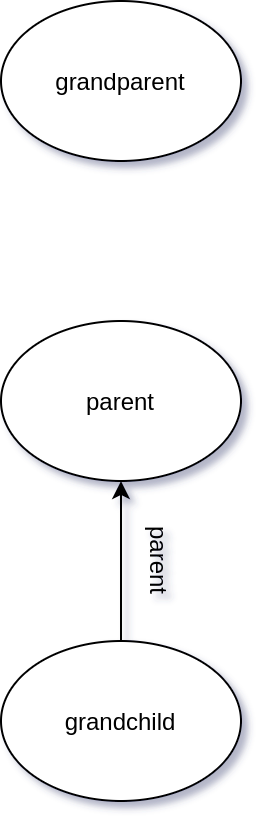
\includegraphics[height=50mm, keepaspectratio]{figures/basic-pattern-explanation-2.png}
\caption{The \texttt{parent} entity, in parent relation with \texttt{grandchild}}
\label{fig:basic-pattern-explanation-2}
\end{figure}

Finally, the second line declares a parent relation between \texttt{parent} and
\texttt{grandparent}, finishing the grandparent pattern.

\begin{figure}[!htbp]
\centering
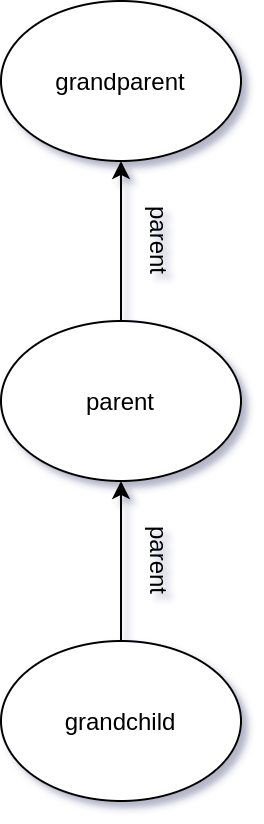
\includegraphics[height=50mm, keepaspectratio]{figures/basic-pattern-explanation-3.png}
\caption{Complete grandparent-grandchild pattern}
\label{fig:basic-pattern-explanation-3}
\end{figure}

\subsection{Evaluating patterns}
Let's see an example of this pattern being matched on a model. Let's say we have
a minimalistic node tree, shown below.

\begin{figure}[!htbp]
\centering
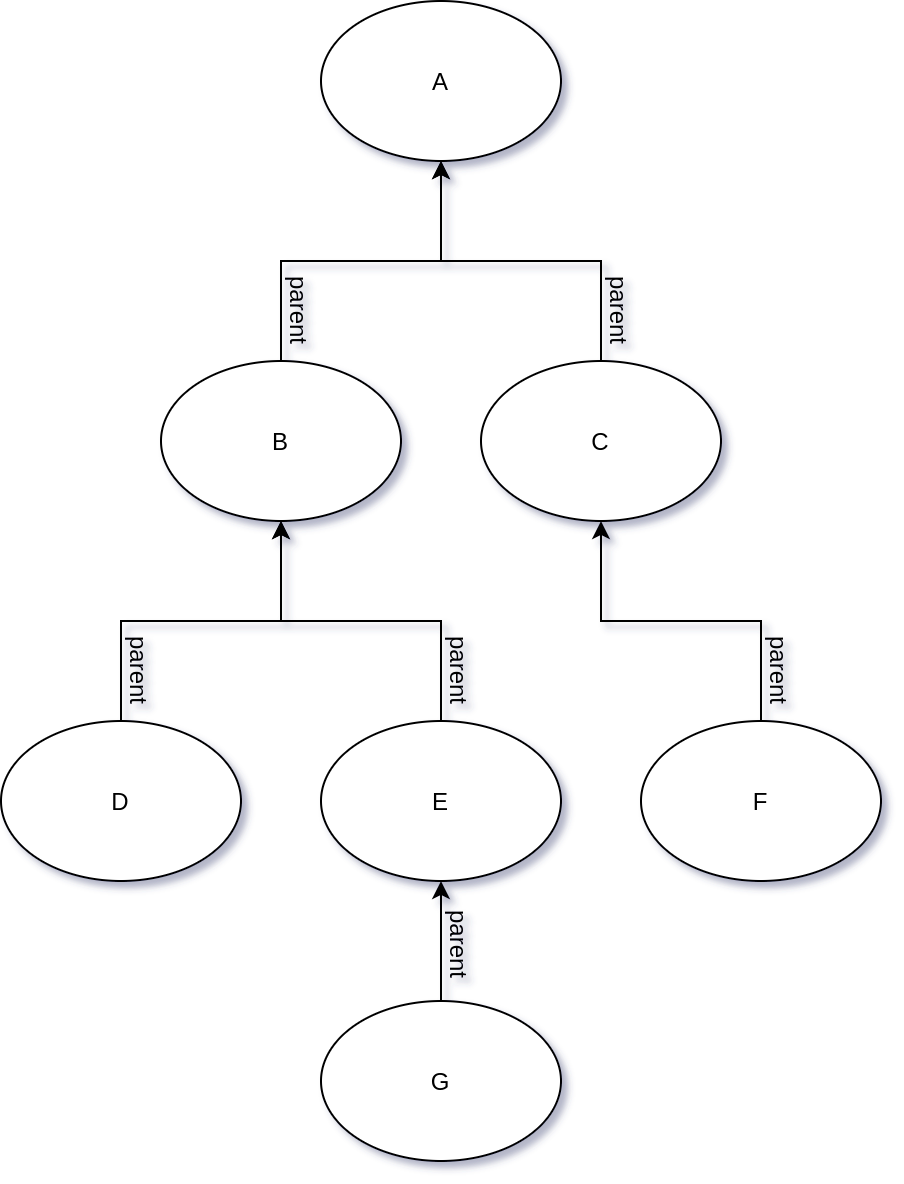
\includegraphics[height=100mm, keepaspectratio]{figures/basic-eval-explanation-1.png}
\caption{A basic node tree model}
\label{fig:basic-eval-explanation-1}
\end{figure}

In this model, matching the \texttt{grandparentOf} pattern will give us four
results: A is the grandparent of D, E, and F, and B is the grandparent of G.

\begin{figure}[!htbp]
\centering
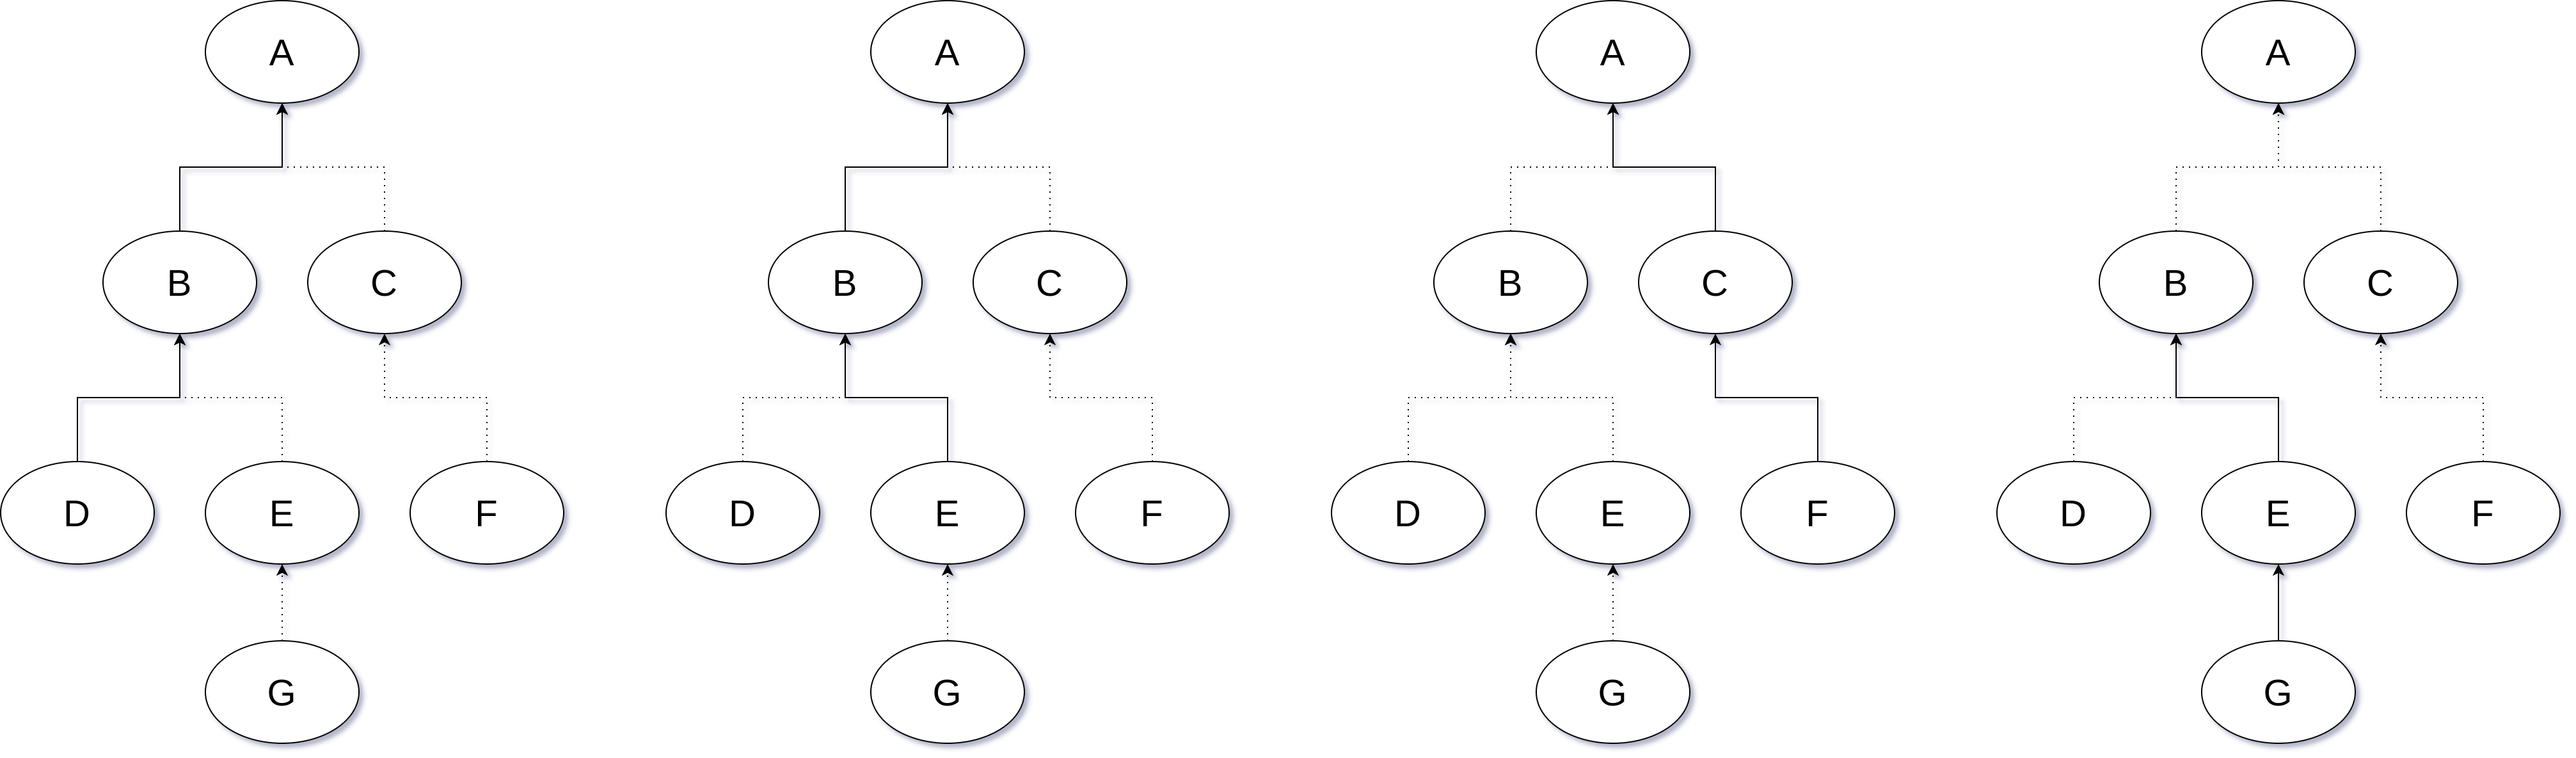
\includegraphics[width=150mm, keepaspectratio]{figures/basic-eval-explanation-2.png}
\caption{The grandparent relations in the above model}
\label{fig:basic-eval-explanation-2}
\end{figure}

\subsection{Pattern disjunction and composition}
Patterns can have multiple declarations, and match other patterns by using the
\texttt{find} keyword.

Let's expand our model: instead of \texttt{Node}s with one parent each, let's
have \texttt{Person} entities, with a separate mother and father. In this case
we can use \textbf{pattern disjunction} to match either parent of a
\texttt{Person}.

\begin{lstlisting}[caption={Parent-child relation, using pattern dijunction}, frame=single]
pattern parentOf(child : Person, parent : Person) {
    Person.mother(child, parent);
} or {
    Person.father(child, parent);
}
\end{lstlisting}

Now we don't have a parent relation, but we do have a pattern, which matches
every parent of a \texttt{Person}. We can use \textbf{pattern composition} to
re-use our previously defined pattern(s).

\begin{lstlisting}[caption={Grandparent-grandchild relation, using pattern composition}, frame=single]
pattern grandparentOf(grandchild : Person, grandparent : Person) {
    find parentOf(grandchild, parent);
    find parentOf(parent, grandparent);
}
\end{lstlisting}

\subsection{Pattern aggregation}
Another language feature frequently used is aggregation. You can use
aggregators for numeric results like \textbf{count}, \textbf{max}, \textbf{min},
and \textbf{sum}. This snippet counts the amount of grandparents a person has.

Any parameter with a single underscore denotes it as a known unused parameter.
In this example, we don't use the \texttt{Person} entities of the grandparents
for anything other than counting them.

\begin{lstlisting}[caption={Counting grandparents using pattern aggregation}, frame=single]
pattern grandparentAmount(child : Person, amount) {
    amount == count find grandparentOf(child, _);
}
\end{lstlisting}

\subsection{Checking and evaluating expressions}
Expression evaluation lets users compute Xbase expressions, allowing calculations.

\begin{lstlisting}[caption={Calculating a \texttt{Person}'s full name using expression evaluation}, frame=single]
pattern fullName(person : Person, name) {
    name == eval(person.firstName + " " + person.lastName);
}
\end{lstlisting}

Additional constraints can be introduced with the \texttt{check} keyword. This
is semantically equivalent to declaring an evaluated expression to be
\texttt{true}.

\begin{lstlisting}[caption={A simple constraint, checking if a \texttt{Person} is an adult}, frame=single]
pattern isAdult(person : Person) {
    check(person.age >= 18);
}
\end{lstlisting}

\subsection{Formulating constraints}
One can also provide model validation, by writing \textbf{constraint patterns}.
This can be done by annotating our validation pattern.

\begin{lstlisting}[caption={Validation constraint, emitting an error message if two \texttt{Person} entities have both parent-child and grandparent-grandchild relations}, frame=single]
@Constraint(targetEditorId = "org.dfintha.familytree",
            severity = "error",
            message = "Person is both a parent and grandparent of someone.",
            key = {"parent"})
pattern bothParentAndGrandparent(person : Person, parent : Person) {
    find parentOf(person, parent);
    find grandparentOf(person, parent);
}
\end{lstlisting}

\section{Implementation details of VQL language services}

\subsection{Validation process}
To validate our query, the Xtext framework parses the query written in VQL
(partially utilizing VIATRA's code), creates a document object model (DOM) of
it, and finally, runs checks on said model. The process of building this DOM is
calling the \texttt{IDerivedStateComputer.installDerivedState} function in the
Xtext framework, which is responsible for producing the current state of our
query.

\begin{figure}[ht]
\centering
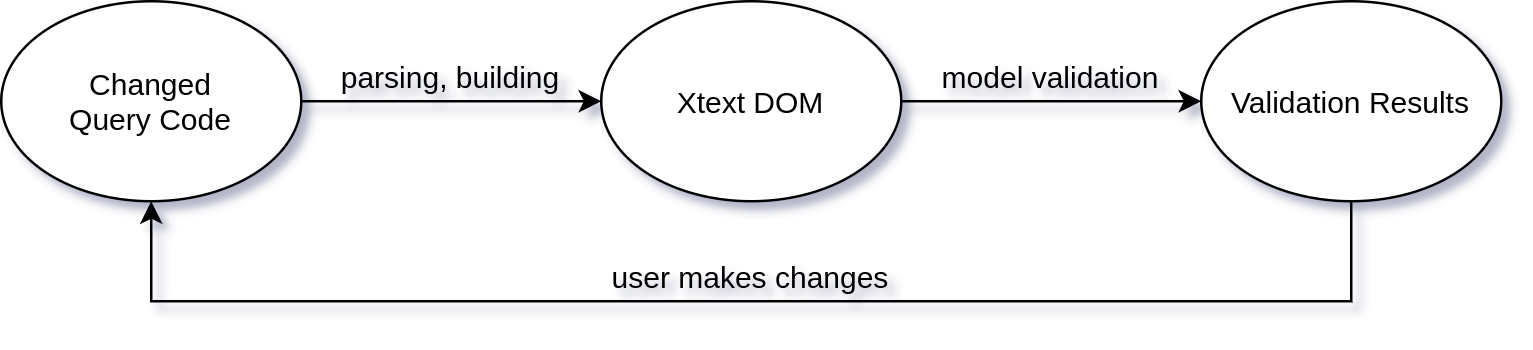
\includegraphics[width=150mm, keepaspectratio]{figures/xtext-validation-process.png}
\caption{The Xtext validation process}
\label{fig:xtext-validation-process}
\end{figure}

The slowest part of this process is building the DOM from the parsed query code.
During model building, the types of variables must be interpreted, and while
most of these variables have an explicitly \textbf{declared type}, type
declaration is optional. VIATRA Query has to \textbf{infer the types of
implicitly-types variables} based on the expressions they are used in.

\begin{lstlisting}[caption={A pattern with variables of both declared and inferred types}, frame=single]
pattern grandparentCount(person : Person, grandparents) {
    grandparents = count find grandparentOf(person, _);
}
\end{lstlisting}

In this small example, the \texttt{person} variable has an explicitly declared
type of \texttt{Person}, but the type of \texttt{grandparents} must be inferred.

\subsection{Automatic update of target platform metamodel}\label{subsec:MetamodelUpdate}
The VIATRA framework is commonly used during plug-in development, providing
services to validate models. As such, it is common that the metamodel of these
models changes along with the query code.

Currently metamodel changes can not be tracked, resulting in periodical checks
for them. This is implemented in the
\texttt{TargetPlatformMetamodelsIndex.update()} function.

Since this caused performance issues, there is an experimental switch to disable
this functionality and use the cached state of metamodels, however, this may
cause incorrect functionality if the metamodel did change.

\chapter{Finding the cause of the editor slowdown}

\section{Setting up a work environment}

\subsection{Eclipse Platform for VIATRA development}
VIATRA, as an Eclipse plugin is developed in Eclipse itself. As such, I needed
an Eclipse environment to develop it. Normally, this should be a straightforward
process, utilizing the Eclipse Oomph installer, but at the time I did my
research the installer didn't work as expected, so I had to install the required
plugins, and add the VIATRA source code to my environment manually.

The detailed steps on how to do this is is written down on the VIATRA project
website\cite{ujhelyi_harmath_david_nagy_hegedus_2019}.

During my work, instead of installing the whole VIATRA framework, I've only
used the relevant components of VIATRA Query their dependencies, avoiding any
unrelated functionality.

\subsection{YourKit Java Profiler}
Since the main issue we have to investigate is a slowdown, I had to use a
profiler software to examine various aspects of software execution, like how
much CPU time did we spend in functions, and how many times functions were
called. Measured data is then compiled into a snapshot, on which one can perform
further analysis.

YourKit Java Profiler has three modes of profiling.
\begin{itemize}
    \item{\textbf{sampling}: measures the time spent in each function}
    \item{\textbf{call count}: measures the amount of times individual functions were called}
    \item{\textbf{tracing}: measures both time spent in functions and call counts}
\end{itemize}

\begin{table}[ht]
    \footnotesize
    \centering
    \begin{tabular}{ l l l }
        \toprule
        Mode & Measures Taken & Overhead \\
        \midrule
        Sampling & Time spent in individual functions & Moderate \\
        Call Count & Times individual functions were called & Low \\
        Tracing & Both time spent and call counts of functions & High \\
        \bottomrule
    \end{tabular}
    \caption{Profiling modes of YourKit Java Profiler}
    \label{tab:profiler-modes}
\end{table}

When using the tracing mode, we also have to opportunity to turn
\textbf{adaptive tracing} on, which ignores measuring trivially fast functions,
reducing the potential overhead it might cause.

\begin{figure}[ht]
\centering
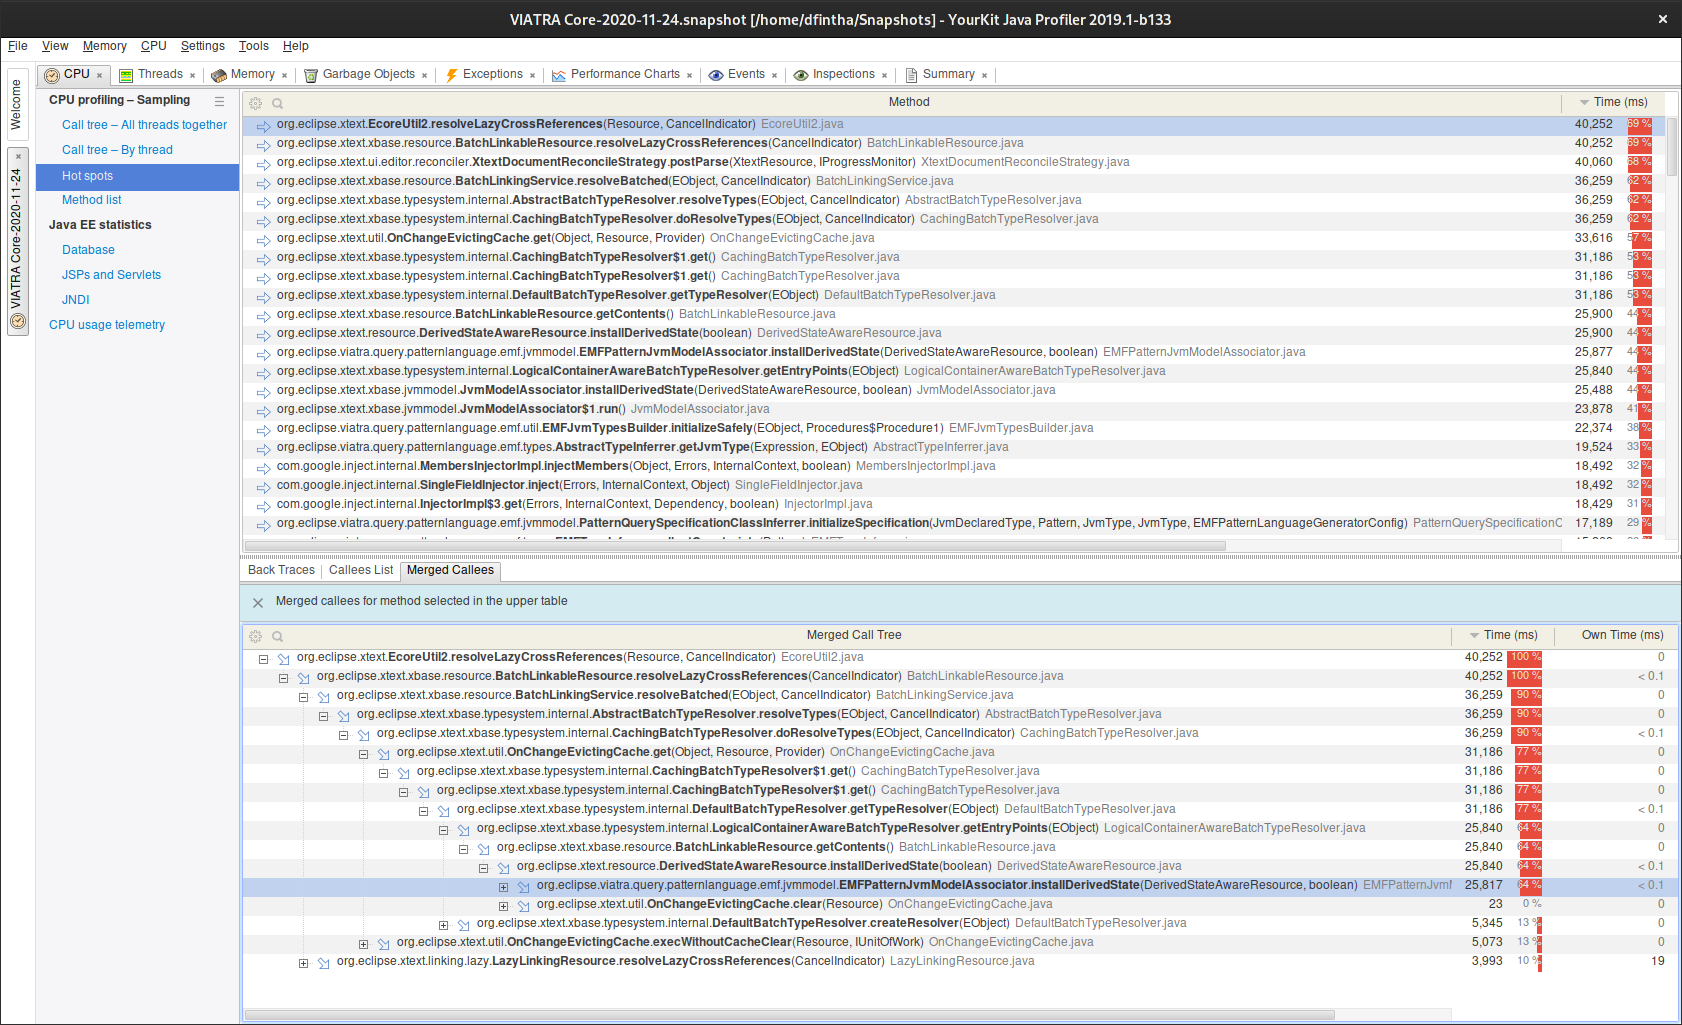
\includegraphics[width=150mm, keepaspectratio]{figures/yourkit-profiler.png}
\caption{YourKit Java Profiler in action}
\label{fig:yourkit-profiler}
\end{figure}

The profiler lets us see the call tree of the profiled software or a list of its
called functions ordered by the time spent in them. It also has a ``hot spots''
mode, which highlights the costliest functions. For each function, we can also
check their backtraces, their callees, and a merged callee list, showing
in-depth information about its callees.

The above figure shows such a merged callee list of a function highlighted in
the ``hot spots'' mode.

\section{Creating a test candidate}
To begin my work, I had to create a test project with a query, which
consistently struggles with such performance issues. The VIATRA-Generator
project\cite{github-viatra-generator} did contain a generated query file, which
had more than enough issues to slow down the workflow.

After having a proper candidate, I had to create a VIATRA
project\cite{github-viatra-vql-slowdown-example} around it, and
remove duplicated pattern code, which existed because of the generated nature
of this query. The finished query did not contain any errors, but caused massive
slowdowns -- it was perfect for my cause.

Before measuring anything with a profiler, I've conducted some manual testing,
which consisted of smaller editing sessions.

\section{Profiling the query language editor}
\subsection{Declaring a profiling workflow}
First of all, I had to create a profiling workflow, which precisely describes
the steps taken to profile the software. Following a fixed workflow ensures that
the measured data will not contain unrelated parts of the software execution,
and will always represent the same steps taken.

\begin{enumerate}
    \item{Start VIATRA in profiling mode, but without starting profiling itself.}
    \item{Wait for Eclipse to start and finish initial tasks.}
    \item{Open the query file, and wait for it to completely load, and highlight syntax.}
    \item{Navigate to a certain pattern (\texttt{mustInstanceOfEClassifier\_class}).}
    \item{\textbf{Start profiling in the profiler software.}}
    \item{Paste the pattern same pattern, with a different name (\texttt{mustInstanceTest}).}
    \item{Wait for the Xtext validation process to finish.}
    \item{\textbf{Stop profiling in the profiler software, and save a snapshot.}}
    \item{Repeat steps 5-8 until I have a sufficent amount of snapshots (10).}
    \item{Quit Eclipse, discarding any changes we made in the file.}
\end{enumerate}

\subsection{Profiling with default settings}
Having a sound profiling plan, I started profiling the software. During my
first profiling session, I did notice the hangups, when I edited the query. This
session provided me with the following suspicious function trail. Each row of
one or more functions in this table was called by the one before it. Rows with
bold font are representing functions inside the VIATRA code base. It should also
be noted, that the contents of these tables are averaged values of 10 separate
measures.

We spent most of the time in the
\texttt{XtextDocumentReconcileStrategy.postParse} function, 71\% of the total
run time on average. The table below gives detailed information about which
functions called by \texttt{postParse} were the most costly.

\begin{table}[ht]
    \footnotesize
    \centering
    \begin{tabular}{ l c }
        \toprule
        Function & Average Time \\
        \midrule
        XtextDocumentReconcileStrategy.postParse & 71\%, 6770 ms \\
        (Xtext framework functions) & - \\
        \textbf{EMFPatternJvmModelAssociator.installDerivedState} & 63\%, 6055 ms \\
        JvmModelAssociator.installDerivedState & 63\%, 6055 ms \\
        JvmModelAssociator\$1.run & 63\%, 5991 ms \\
        (JvmModelAssociator\$1.run callees) & - \\
        \textbf{AbstractTypeInferrer.getJvmType} & 61\%, 5871 ms \\
        (AbstractTypeInferrer.getJvmType callees) & - \\
        \textbf{CompoundMetamodelProviderService.getQualifiedClassName} & 55\%, 5285 ms \\
        \bottomrule
    \end{tabular}
    \caption{Function run times with default settings}
    \label{tab:postparse-default}
\end{table}

The EMFPatternLanguageJvmModelInferrer calls multiple lambdas, but the ones
responsible for most time spent in them are all calling the
\texttt{AbstractTypeInferrer.getJvmType} method, which is responsible for their
long run time. In a similar fashion, most of the time spent in
\textbf{AbstractTypeInferrer.getJvmType} was actually used up not by its
direct callees, but
\textbf{CompoundMetamodelProviderService.getQualifiedClassName} through them.

It should be noted, that the
\texttt{CompoundMetamodelProviderService.getQualifiedClassName} is only called
during metamodel update (explained in section \ref{subsec:MetamodelUpdate}). As
such, I did another profiling session, with the automatic update feature turned
off.

\subsection{Profiling without automatic update of target platform metamodels}
After turning off automatic platform metamodel updates, we can have more concise
profiling results with less noise. Repeating the same process yielded the
following, slightly different results. Now the
\texttt{XtextDocumentReconcileStrategy.postParse} function only took 38\% of the
total run time on average, and the responsiveness of the application was
significantly better.

\begin{table}[ht]
    \footnotesize
    \centering
    \begin{tabular}{ l c }
        \toprule
        Function & Average Time \\
        \midrule
        XtextDocumentReconcileStrategy.postParse & 38\%, 1707 ms \\
        (Xtext framework functions) & - \\
        \textbf{EMFPatternJvmModelAssociator.installDerivedState} & 21\%, 960 ms \\
        JvmModelAssociator.installDerivedState & 21\%, 960 ms \\
        JvmModelAssociator\$1.run & 19\%, 875 ms \\
        (JvmModelAssociator\$1.run callees) & - \\
        \textbf{AbstractTypeInferrer.getJvmType} & 16\%, 725 ms \\
        \textbf{AbstractTypeInferrer.getType} & 13\%, 562 ms \\
        \bottomrule
    \end{tabular}
    \caption{Function run times without automatic metamodel updates}
    \label{tab:postparse-no-auto-update}
\end{table}

Although some performance improvements could be noticed, editor hangups still
happen. Now \texttt{AbstractTypeInferrer.getType} is the most expensive function
called by \textbf{AbstractTypeInferrer.getJvmType}.

In conclusion, metamodel updates are very costly, and even though turning
automatic updates off does save some time, expensive calculations still happen
frequently and should be optimized. My next step was to understand the code
responsible for type inference, and look for opportunities to optimize it.

My choice of optimization is implementing a cache for the
\texttt{AbstractTypeInferrer}, to avoid repeated inferences of the same type.
Since it takes a large part of the run time (33\% without automatic update,
and 75\% with it), the speedup should be significant.

\chapter{Fixing performance issues}
In this chapter, I'll present three separate opportunities to increase the
performance of VQL tooling.

\section{Implementing a type inferrer cache}
\subsection{Inspecting the original functionality}
During the type inference process, \texttt{getJvmType} is called numerous times,
resulting in a massive amount of processing time (more than 6 seconds) spent
there. Let us see, how this function works.

\begin{lstlisting}[caption={Original source code of \texttt{getType}}, language=java]
// ...

/**
 * @since 1.3
 */
@Override
public IInputKey getType(Expression ex) {
    final IInputKey declaredType = getDeclaredType(ex);
    if (declaredType != null) {
        return declaredType;
    } else {
        return getInferredType(ex);
    }
}

//...

/**
 * @since 1.3
 */
@Override
public JvmTypeReference getJvmType(Expression ex, EObject context) {
    return typeSystem.toJvmTypeReference(getType(ex), context);
}

// ...
\end{lstlisting}

The profiling session showed us that we spend most of the time in the
\texttt{getType} function, and inside that, the \texttt{getInferredType}
function, which actually does a costly type calculation, and does so repeatedly.
This looks like a good candidate for some caching mechanism.

\subsection{Caching computed results}
My approach was using a cache in the \texttt{AbstractTypeInferrer} class,
which was implemented in the \texttt{TypeInformation} class. This cache
stores the types (\texttt{IInputKey}) of \texttt{Expression} objects. This
cache is invalidated by each change in the file, but helps avoid repeated
calculations during each pass.

The following significant changes were made to the source code.

\begin{lstlisting}[caption={AbstractTypeInferrer.java}, language=java]
// ...

/**
 * @since 1.3
 */
@Override
public IInputKey getType(Expression ex) {
    TypeInformation typeInformation = getTypeInformation(ex);
    return typeInformation.getOrComputeType(ex, expression -> {
        final IInputKey declaredType = getDeclaredType(expression);
        if (declaredType != null)
             return declaredType;
        return getInferredType(expression);
    });
}

// ...

protected abstract TypeInformation getTypeInformation(final EObject element);

// ...
\end{lstlisting}

\begin{lstlisting}[caption={TypeInformation.java}, language=java]
// ...

final Map<Expression, IInputKey> typeComputed = new HashMap<>();

// ...

public IInputKey getOrComputeType(Expression expression, Function<? super Expression, ? extends IInputKey> computation) {
    return typeComputed.computeIfAbsent(expression, computation);
}

// ...
\end{lstlisting}

The \texttt{TypeInformation} class did already contain cache for some computed
values, so I've ended up extending it with this mapping, too. Because the
lifetimes of \texttt{TypeInformation}s are already well-defined, I did not have
to write any code to clear my cache.

\subsection{Comparing the optimized state with the original one}
After making these changes, I did another profiling session, with the same
workflow described above. Seemingly my solution did not fully accomplish my
goal, since the run time of the validation process remained close to the same.
The \texttt{XtextDocumentReconcileStrategy.postParse} function still ate up 35\%
of the run time (compared to the original 38\%), but the type inference code
became very slightly faster.

\begin{table}[ht]
    \footnotesize
    \centering
    \begin{tabular}{ l c c }
        \toprule
        Function & Avg. Time (Before) & Avg. Time (After) \\
        \midrule
        XtextDocumentReconcileStrategy.postParse & 38\%, 1707 ms & 35\%, 1687 ms\\
        (Xtext framework functions) & - \\
        \textbf{EMFPatternJvmModelAssociator.installDerivedState} & 21\%, 960 ms & 21\%, 888 ms \\
        JvmModelAssociator.installDerivedState & 21\%, 960 ms & 21\%, 888 ms \\
        JvmModelAssociator\$1.run & 19\%, 875 ms & 19\%, 819 ms \\
        (JvmModelAssociator\$1.run callees) & - \\
        \textbf{AbstractTypeInferrer.getJvmType} & 16\%, 725 ms & 16\%, 681 ms \\
        \textbf{AbstractTypeInferrer.getType} & 13\%, 562 ms & 12\%, 519 ms \\
        \bottomrule
    \end{tabular}
    \caption{Function run times without automatic metamodel updates}
    \label{tab:postparse-no-auto-update}
\end{table}

The time spent in functions called by the \texttt{getType} function did not
significantly decrease. The purpose of my cache was minimizing calls to the
\texttt{getInferredType} function, which took the most time. However, the
average amount of time spent there was roughly the same (562 and 519
milliseconds, respectively).

To make sure that hashing two \texttt{Expression} objects representing the same
expression do produce identical hashes, I did a single pass of profiling in
tracing mode, to see how many times did we have to call either
\texttt{getInferredType} or \texttt{getDeclaredType} because of a cache miss.
Call count percentages are rounded to two digits.

\begin{table}[ht]
    \footnotesize
    \centering
    \begin{tabular}{ l c c c }
        \toprule
        Function & Count & Count (\%) \\
        \midrule
        (total calls to getType) & 12368 & 100\% \\
        EMFTypeInferrer.getInferredType & 63 & 0.51\% \\
        EMFTypeInferrer.getDeclaredType & 1357 & 10.97\% \\
        \bottomrule
    \end{tabular}
    \caption{Time and call count of callees of \texttt{getType} with my solution}
    \label{tab:first-solution-call-counts}
\end{table}

To also make sure that it was my addition that prevented the redundant calls, I
did a similar profiling session with the original source code, too. Please note,
that the reason, why the amount of \texttt{getDeclaredType} calls is less than
the amount of \texttt{getType} is that the process was interrupted.

\begin{table}[ht]
    \footnotesize
    \centering
    \begin{tabular}{ l c c c }
        \toprule
        Function & Time (\%) & Count & Count (\%) \\
        \midrule
        (total calls to getType) & 100\% & 12584 & 100\% \\
        EMFTypeInferrer.getInferredType & 97\% & 138 & 1.10\% \\
        EMFTypeInferrer.getDeclaredType & 3\% & 12583 & 100.00\% \\
        \bottomrule
    \end{tabular}
    \caption{Time and call count of callees of \texttt{getType} with the original source}
    \label{tab:first-solution-call-counts}
\end{table}

The results of these trace mode profilings have proven my suspicion false. The
most part of the \texttt{getType} function was still spent in
\texttt{getInferredType}, but my cache did help avoid some repeated
calculations.

To see how much memory did my cache use, I've made a memory snapshot of the
modified state. In this snapshow the \texttt{TypeInformation} class only took
3 megabytes of memory (including my cache). As such, its memory consumption did
not raise any problems.

\subsection{Profiling results}
To compare the profiling results original and the modified source code, I did
separate profiling sessions with 10 measurements of each case:
\begin{itemize}
    \item{the original source code with default settings,}
    \item{the original source code without automatic platform metamodel updates,}
    \item{and the modified source code without automatic platform metamodel updates}
\end{itemize}

In the following figure, each table represents one of these cases (noted on the
top left corner), each row represents either the time spent in a function, or
the percentage of total time spent there, and each column is a separate
measurement. The rightmost column contains the averages of the values.

\begin{figure}[ht]
\centering
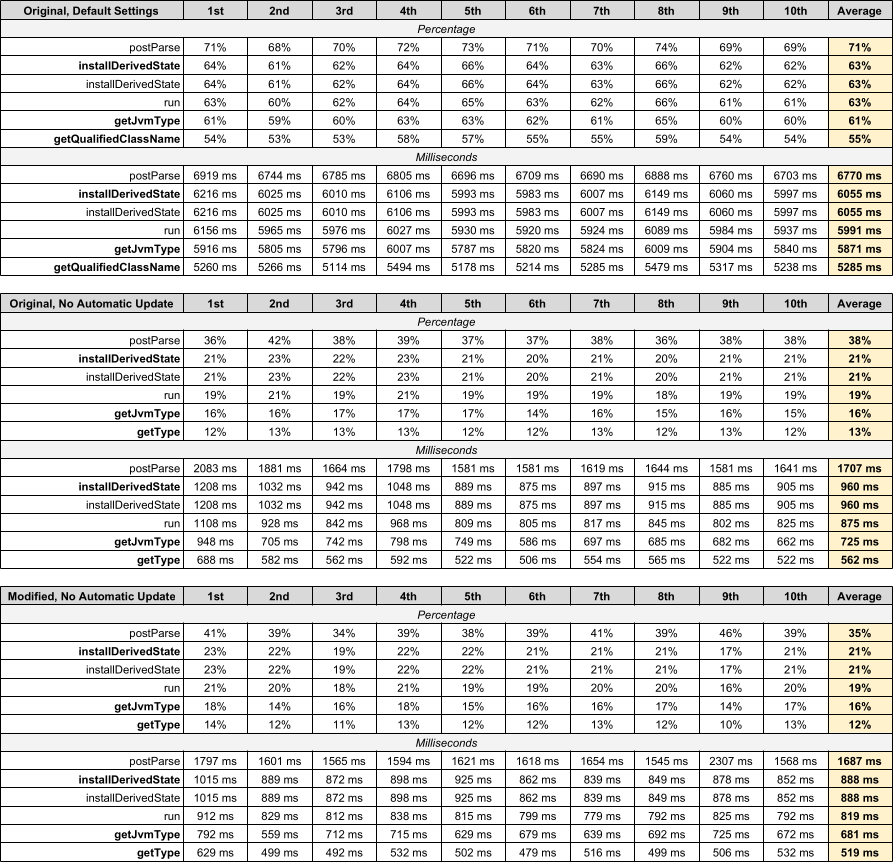
\includegraphics[width=150mm,keepaspectratio]{figures/measurements.png}
\caption{Profiling results with calculated averages}
\label{fig:profiling-measurements}
\end{figure}

\subsection{Conclusion}
If we look back at the previous implementation of \texttt{getType}, we can see
that \texttt{getDeclaredType} was called the same amount of times as
\texttt{getType} itself, but if it failed, we fell back to
\texttt{getInferredType} After adding the type cache, the call count of the two
functions added dropped to only 11.48\% of the total call count.

However, the fact that this caching mechanism did not result in a significant
speedup indicates, that other caching mechanisms of the functions responsible
for type inference already help us avoid the most costly calculations.

\section{Fine-grained type caching}\label{sec:FineGrained}
Caching the calculated types did accomplish a minor speedup, but the editor
still hangs up during Xtext validation.

The Xtext framework caches information during file processing in a cache, but as
soon as the file is changed, the cache is evicted, and this information is lost.
My additional type cache helped keep some values cached \textbf{during this
processing, avoiding re-calculation of the same type in one process}, but some
of the values still need to be recalculated.

To further optimize the process, these calculated types for expressions could
be kept in a cache that persists between changed states, as long as the parts of
the file relevant to them did not change. This could result in an additional
significant speedup.

Looking for such a cache mechanism, I studied the Xtext framework documentation
for a cache other than \texttt{OnChangeEvictingCache}, but on developer forums,
it was stated to be nonexistent, and extremely complex to
implement\cite{xtext-fine-grained-caching}. As such, I had to look for another
solutions.

\section{Improving type inference performance}
During type inference, the \texttt{EMFTypeInferrer.collectConstraints} function,
which takes up the most time in \texttt{getInferredType}, does repeated type
calculations of patterns. This is done in a loop, which first queries and filter
referenced patterns, and after that, if the subject pattern wasn't already
processed, does type inference.

Here is the source code of the \texttt{EMFTypeInferrer.collectConstraints}
function. \texttt{PatternLanguageHelper.getReferencedPatterns} is always called
in the for loop, even if \texttt{patternToCheck} was already processed.

\begin{lstlisting}[caption={Original source code of \texttt{collectConstraints}}, language=java]
private TypeInformation collectConstraints(final Pattern pattern) {
    final TypeInformation types = cache.get(this, pattern.eResource(), () -> new TypeInformation(typeSystem));

    // XXX requiring an ordered call graph might be expensive, but it avoids inconsistent errors during type inference
    // The UNTYPED_PARAMETER_PREDICATE is used to return a reduced call graph where pattern with only declared types are (transitively) ignored.
    final Set<Pattern> patternsToCheck = PatternLanguageHelper.getReferencedPatternsTransitive(pattern, true, NON_NULL.and(UNTYPED_PATTERN_PREDICATE));
    patternsToCheck.add(pattern);

    for (Pattern patternToCheck : patternsToCheck) {
        PatternLanguageHelper.getReferencedPatterns(patternToCheck).stream()
            .filter(NON_NULL.and(TYPED_PATTERN_PREDICATE))
            // Ensure called parameter types are loaded
            .forEach(typedCall -> rules.loadParameterVariableTypes(typedCall, types));
        if (!types.isProcessed(patternToCheck)) {
            rules.inferTypes(patternToCheck, types);
            for (PatternBody body : patternToCheck.getBodies()) {
                for (Iterator<EObject> it = body.eAllContents(); it.hasNext();) {
                    EObject obj = it.next();
                    if (obj instanceof Constraint || obj instanceof Expression) {
                        rules.inferTypes(obj, types);
                    }
                }
            }
            types.setProcessed(patternToCheck);
        }

    }

    return types;
}
\end{lstlisting}

A potential problem was that even if the subject pattern was already processed,
we still query and filter its referenced patterns, causing potentially redundant
calculations.

In this part, I made a simple change in the loop to avoid any calculations on
already processed patterns.

\begin{lstlisting}[caption={Modified source code of \texttt{collectConstraints}}, language=java]
private TypeInformation collectConstraints(final Pattern pattern) {
    final TypeInformation types = cache.get(this, pattern.eResource(), () -> new TypeInformation(typeSystem));

    // XXX requiring an ordered call graph might be expensive, but it avoids inconsistent errors during type inference
    // The UNTYPED_PARAMETER_PREDICATE is used to return a reduced call graph where pattern with only declared types are (transitively) ignored.
    final Set<Pattern> patternsToCheck = PatternLanguageHelper.getReferencedPatternsTransitive(pattern, true, NON_NULL.and(UNTYPED_PATTERN_PREDICATE));
    patternsToCheck.add(pattern);

    for (Pattern patternToCheck : patternsToCheck) {
        if (types.isProcessed(patternToCheck))
            continue;

        PatternLanguageHelper.getReferencedPatterns(patternToCheck).stream()
            .filter(NON_NULL.and(TYPED_PATTERN_PREDICATE))
            // Ensure called parameter types are loaded
            .forEach(typedCall -> rules.loadParameterVariableTypes(typedCall, types));
        rules.inferTypes(patternToCheck, types);
        for (PatternBody body : patternToCheck.getBodies()) {
            for (Iterator<EObject> it = body.eAllContents(); it.hasNext();) {
                EObject obj = it.next();
                if (obj instanceof Constraint || obj instanceof Expression) {
                    rules.inferTypes(obj, types);
                }
            }
        }
        types.setProcessed(patternToCheck);
    }

    return types;
}
\end{lstlisting}

However, after a profiling session, I did not find any measurable performance
differences.

\chapter{Summary}

During my work, I've looked into into the depths of VIATRA Query's process of
parsing query code, and searched for ways to improve its performance. After
detailed analysis, I could not find any way to significantly increase the
tooling performance, unless one can extend the functionality of the Xtext
language framework, on top of which VIATRA Query was implemented.

Sadly, the improvements made by my caching mechanisms were miniscule. As such,
it was not published to the mainstream code base.

\section{Improvement opportunities}

\subsection{Fine-grained cache for the Xtext framework}
As seen in \ref{sec:FineGrained}, a cache, which could keep patterns stored
between query changes could by itself cause a significant performance
improvement. However, this is an extremely complex task.

\subsection{Caching qualified type names}
When automatic target platform metamodel updates were turned on, the
\texttt{CompoundMetamodelProviderService.getQualifiedClassName} function ate up
most of the time. The problem with caching these, is that we have to iterate
over each metamodel, and that process can not be cached. However, we could avoid
repeatedly iterating over metamodels during validation, by disabling the
automatic update feature at the start of the process, and re-enabling it when it
ends.

This issue can be worked around by turning updates off in the VIATRA tooling
settings.

% ---------------------------------------------------------------------------- %

\listoffigures\addcontentsline{toc}{chapter}{\listfigurename}
\listoftables\addcontentsline{toc}{chapter}{\listtablename}
\addcontentsline{toc}{chapter}{\bibname}
\bibliography{bib/mybib}
\label{page:last}

\end{document}
